\documentclass[aspectratio=169]{beamer}
\usepackage{xcolor}
\usepackage{tikz}
\usetikzlibrary{patterns}
\usepackage{amsmath, amssymb, bm}

% settings for the beamer theme
\usetheme[progressbar= frametitle]{metropolis}
\setbeamertemplate{frame numbering}[fraction]
\useoutertheme{metropolis}
\useinnertheme{metropolis}
\usecolortheme{spruce}
\setbeamercolor{background canvas}{bg=white}
\definecolor{mygreen}{rgb}{.125, .5, .125}
\usecolortheme[named=mygreen]{structure}

% setting for the title
%\title[Short Title]{Beamer-Krumel}
\title{Elementos Básicos de Teoría de Conjuntos}
%\subtitle{Subtitle Here}
\usepackage{graphicx} % Required for inserting images
%\author{Kenyer Aguiar}
%\institute{Institute}
\institute{\large\textbf{Objetivo de la clase:} \\[6pt]
Comprender el concepto de conjunto y realizar operaciones básicas con conjuntos.}
\date{}

\begin{document}
% filling for blocks
\metroset{block=fill}

\begin{frame}
\titlepage  
\end{frame}


\begin{frame}[t]{Motivación}\vspace{30pt} % addign vertical space
\begin{block}{Preguntas}
\vspace{0.5em}
\begin{enumerate}
    \only<1->{\item ¿Cómo agruparías a los estudiantes que practican fútbol, los que tocan instrumentos y los que hacen ambas cosas?}
    \only<2->{\item ¿Podemos agrupar objetos por características?}
    \only<3->{\item ¿De qué manera podemos representar lo anterior de manera gráfica?}
\end{enumerate}
    


\vspace{0.5em}
\end{block}
\vspace{10pt}


\end{frame}

\begin{frame}[c]{Conjuntos}\vspace{2pt} % addign vertical space
\begin{block}{Definición}
\vspace{0.5em}
    Un \textbf{{conjunto}} es una colección \textbf{bien definida} de objetos llamados \textbf{elementos}.
\vspace{0.5em}
\end{block}
\vspace{10pt}
\only<2->{
\begin{block}{Ejemplos}
\vspace{0.5em}
    \begin{itemize}
        \only<2->{\item Conjunto de estudiantes del curso.}
        \only<3->{\item Conjunto de números pares.}
        \only<4->{\item Conjunto de vocales.}
        \only<5->{\item Conjunto de cantantes favoritos.}
        \only<6->{\item Conjunto de mis amigos.}
    \end{itemize}
\vspace{0.5em}
\end{block}
\vspace{10pt}}

\end{frame}


\begin{frame}[t]{Para Pensar}\vspace{30pt} % addign vertical space
\begin{block}{Pregunta}
\vspace{0.5em}
¿El conjunto de “estudiantes altos” está bien definido?
\end{block}
    
\vspace{10pt}

\end{frame}

\begin{frame}[c]
\frametitle{Notación Básica}
{\Large
\vspace{10pt}
\begin{enumerate}
    \only<1->{\item Los conjuntos \textbf{se nombran con letras mayúsculas} ($\mathbf{A}, \mathbf{B}, \mathbf{C}$).}
    \only<2->{\item Los elementos se \textbf{escriben entre llaves} $\mathbf{\{\dots\}}$.}
    \only<3->{\item \textbf{Pertenencia:} Si $x$ está en $A$, usamos $x \in A$. Si no, $x \notin A$.}
\end{enumerate}
}
\end{frame}

\begin{frame}[t]{Ejemplos}\vspace{30pt} 
\begin{block}{Ejemplo 1}
Escribe el conjunto $S$ de tus cinco series favoritas.
\vspace{30pt} 
\end{block}
\begin{block}{Ejemplo 2}
Escribe el conjunto $A$ de los primeros números 10 números naturales.
\vspace{30pt} 
\end{block}

\end{frame}
\begin{frame}[c]{Conjuntos Numéricos Importantes } 
\Large
\begin{itemize}
    \only<1->{\item Números Naturales: $\mathbb{N} = \{1, 2, 3,4, 5 ...\}$.}
    \only<2->{\item Números Enteros: $\mathbb{Z} = \big\{0, 1, -1, 2, -2, 3, -3, 4, -4, 5, -5, ...\big\}$.}
    \only<3->{\item Números Racionales: $\mathbb{Q} = \left\{\dfrac{a}{b} \textbf{ tales que } a, b\in \mathbb{Z}, b\neq 0\right\}$.}
    \only<4->{\item Números irracionales: Números que no pueden ser escritos como una fracción. Los números irracionales tienen expansión decimal infinita y no periódica. Se denotan por $\mathbb{I}$.}
    \only<5->{\item Números Reales: son el conjunto formado por todos los números racionales y todos los números irracionales. Se denota por $\mathbb{R}$.}
\end{itemize}

\end{frame}


\begin{frame}[t]{Ejemplo de Pertenencia}
\Large
    Complete la tabla usando los símbolos $\in$ ó $\notin$ según corresponda.
    \[
\begin{array}{|c|c|c|c|c|}
\hline
\text{Número} & \mathbb{N} & \mathbb{Z} &\mathbb{Q} & \mathbb{R} \\
\hline
5      &               &               &         &      \\
\hline
-3     &               &               &         &      \\
\hline
0      &               &               &         &      \\
\hline
2.5    &               &               &         &      \\
\hline
\sqrt{2} &             &               &          &     \\
\hline
-7.8   &               &               &          &     \\
\hline
\end{array}
\]

\end{frame}


\begin{frame}[c]{Formas de Especificar un Conjunto}
\huge
\only<1->{Existen dos maneras de especificar los elementos de un conjunto:}

\only<2->{\begin{itemize}
    \only<2>{\item \textbf{Por Extensión}: Listar todos los elementos. Ejemplos:
    \begin{enumerate}
        \item $A=\{a,e,i,o,u\}$.
        \item $C=\{0,1, 2, 3, 4, 5, 6,7, 8, 9\}$
    \end{enumerate}}
    
    \only<3>{\item \textbf{Por Comprensión}: Indicar la propiedad que los define. Ejemplos
    \begin{enumerate}
        \item $D=\{x:x \text{ es una vocal}\}$
        \item $E=\{x: x \text{ es un número par entre 1 y 10}\}$
        \item $F=\{x: x \text{ es un país de sudamérica}\}$
    \end{enumerate}}

\end{itemize}}
\end{frame}

\begin{frame}[t]{Ejemplo}\vspace{30pt}
\Large
Especifica por extensión el siguiente conjunto
$$A= \{x: x\text{ es un planeta del sistema solar} \}$$
\end{frame}

\begin{frame}[t]{Ejemplo}\vspace{30pt} 
\Large
Especifica por extensión el siguiente conjunto
$$C= \{x: x\text{ es un color del arcoíris } \}$$
\end{frame}

\begin{frame}[t]{Ejemplo}\vspace{30pt} 
\Large
Dado el siguiente conjunto
$$A= \{a, e, i , o, u\}.$$ Escribe el conjunto por comprensión.
\end{frame}

\begin{frame}[c]
\frametitle{Conjuntos Especiales} 
{\Large
\begin{itemize}
    \item Conjunto \textbf{Vacío} $\varnothing$ o $\{\}$: No tiene elementos.
    \item Conjunto \textbf{Universo} $U$: El marco de referencia para el problema.
\end{itemize}
}
\end{frame}


\begin{frame}[t]{Diagramas de Venn}
\Large
\only<1->{Un \textbf{diagrama de Venn} es una forma gráfica de representar un conjunto.}
\begin{center}
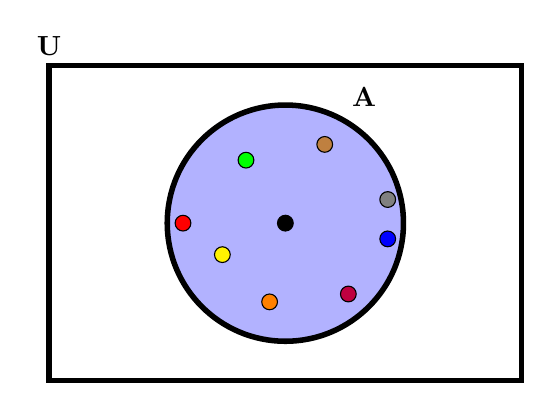
\begin{tikzpicture}
    % Dibujar el rectángulo del universo
    \draw[line width = 2pt] (1,0) rectangle (7,4);
    \node at (1,4)[above] {$\mathbf{U}$}; % Universo

    % Dibujar el círculo del conjunto A
    \draw[line width = 2pt, fill = blue, fill opacity = 0.3] (4,2) circle (1.5);
    \node at (5,3.6) {$\mathbf{A}$};
    % Dibujar elementos del conjunto
   \draw[ fill=black] (4,2) circle (0.1);      % Punto 1
    \draw[ fill=brown] (4.5,3) circle (0.1);    % Punto 2
    \draw[ fill=red] (2.7,2) circle (0.1);    % Punto 3
    \draw[ fill=green] (3.5,2.8) circle (0.1);    % Punto 4
    
    \draw[ fill=gray] (5.3,2.3) circle (0.1);  % Punto 6
    \draw[ fill=blue] (5.3,1.8) circle (0.1);  % Punto 7
    \draw[fill=yellow] (3.2,1.6) circle (0.1);  % Punto 8
    \draw[ fill=orange] (3.8,1) circle (0.1);  % Punto 9
    \draw[fill=purple] (4.8,1.1) circle (0.1);  % Punto 10

\end{tikzpicture}
\end{center}
\end{frame}

\begin{frame}[t]{Ejemplo Venn}
    

\only<1->{\begin{block}{Ejemplo}
Representa gráficamente los siguientes conjuntos
\begin{itemize}
    \item A = \{x: x \text{ es un estudiante de música}\}
    \item B = \{x: x \text{ es estudiante de física}\}
\end{itemize}
\end{block}}
\end{frame}
\begin{frame}[t]{Problema de aplicación}
\Large
En una encuesta, $20$ personas prefieren el fútbol, $15$ prefieren el básquetbol y $5$ prefieren ambos. ¿Cuántas personas prefieren solo fútbol? ¿Cuántas prefieren solo básquetbol?
\end{frame}

\begin{frame}{Subconjuntos}
\large
\begin{block}{Definición}
Sean $A$ y $B$ conjuntos. Diremos que $\mathbf{A}$\textbf{ es subconjunto de} $\mathbf{B}$ 
o que $\mathbf{A}$ \textbf{está incluido en} $\mathbf{B}$, y escribiremos $\mathbf{A \subset B}$, 
si todo elemento de $A$ es también elemento de $B$. 

Esto es, simbólicamente:

\[
\mathbf{A \subset B \Longleftrightarrow (\forall x)(x \in A \; \Rightarrow \;  x\in B)}
\]

\end{block}

\end{frame}
\begin{frame}{Interpretación gráfica de la Contención de Conjuntos}
\begin{center}
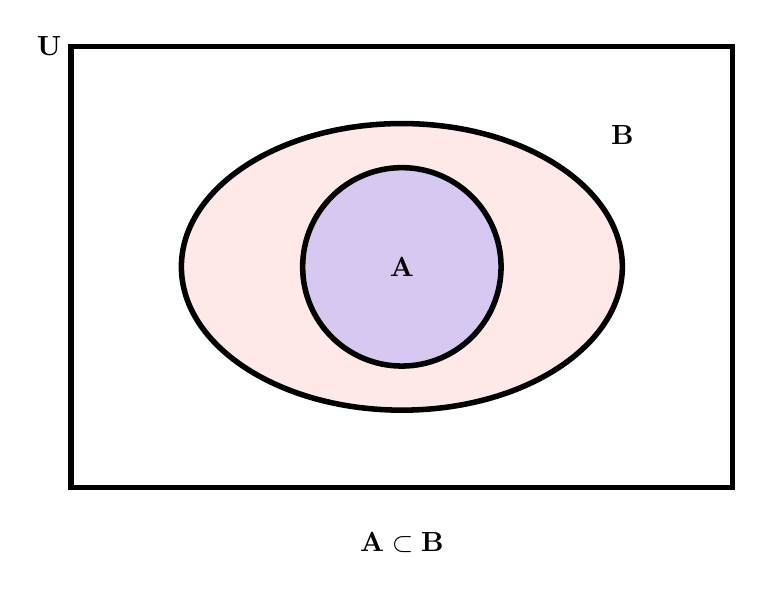
\begin{tikzpicture}[scale=1.4]
% Rectángulo del conjunto universal
\draw[line width=2pt] (1,0) rectangle (7,4);
% Conjunto B (elipse)
\draw[line width=2pt, fill=red!30, fill opacity=0.3] 
(4,2) ellipse (2 and 1.3);

% Conjunto A (círculo dentro de B)
\draw[line width=2pt, fill=blue!40, fill opacity=0.4] 
(4,2) circle (0.9);
% Etiquetas
\node at (1,4)[left] {$\mathbf{U}$};
\node at (4,2) {$\mathbf{A}$};
\node at (6,3.2) {$\mathbf{B}$};

% Texto inferior
\node at (4,-0.5) {$\mathbf{A \subset B}$};

\end{tikzpicture}

\end{center} 
\end{frame}

\begin{frame}[t]{Negación de la Contención}
    A la negación de $A \subset B$ la denotaremos así: $A \not\subset B$.
    \begin{block}{Ejemplo}
    Si $A = \{ 1, 2, 3\}$ y $B = \{ 1, 2, 3, 4, 5 \}$, entonces $A \subset B$ y $B\not\subset  A$.
\end{block}
\begin{block}{Ejercicio}
Completa con el símbolo $ \subset$ ó $\not\subset$ según corresponda.
\begin{columns}[onlytextwidth]
\column{0.5\textwidth}
\begin{itemize}
    \item $\mathbb{N}\,\line(1,0){15}\,  \mathbb{Z}$
    \item $\mathbb{Z}\,\line(1,0){15}\,  \mathbb{N}$
    \item $\mathbb{N}\,\line(1,0){15}\,  \mathbb{R}$
    \item $\mathbb{R}\,\line(1,0){15}\,  \mathbb{N}$
    \item $\mathbb{R}\,\line(1,0){15}\,  \mathbb{R}$
\end{itemize}



\column{0.5\textwidth}
\begin{itemize}
    \item $\mathbb{Q}\,\line(1,0){15}\,  \mathbb{Z}$
    \item $\mathbb{Z}\,\line(1,0){15}\,  \mathbb{Q}$
    \item $\mathbb{Q}\,\line(1,0){15}\,  \mathbb{N}$
    \item $\mathbb{N}\,\line(1,0){15}\,  \mathbb{N}$
    \item $\mathbb{R}\,\line(1,0){15}\,  \mathbb{Z}$
\end{itemize}
\end{columns}
\end{block}
\end{frame}


\begin{frame}[t]{Operaciones con conjuntos}\vspace{30pt}
\Huge
Operaciones con conjuntos
\end{frame}

\begin{frame}[t]{Unión} 
\large
\begin{block}{Definión}
\textbf{La unión} de $A$ y $B$  es el conjunto formado por los elementos que están en $A$, en $B$ o en ambos.
$$A\cup B = \{x: x\in A \text{ o } x\in B\}.$$
\end{block}

\only<2>{\begin{center}
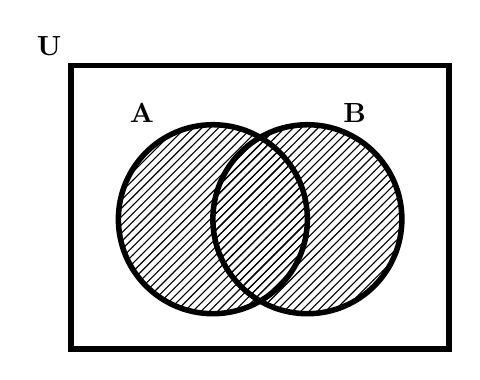
\begin{tikzpicture}[scale=0.6]

\draw[line width=2pt] (0,0) rectangle (8,6);

\draw[line width=2pt] (3,2.75) circle(2); % A
\draw[line width=2pt] (5,2.75) circle(2); % B

\begin{scope}

\clip (0,0) rectangle (8,6);
\fill[pattern=north east lines] (3,2.75) circle(2);
\fill[pattern=north east lines] (5,2.75) circle(2);

\end{scope}

\node at (1.5,5) {$\mathbf{A}$};
\node at (6,5) {$\mathbf{B}$};
\node at (0,6)[above left] {$\mathbf{U}$};

\end{tikzpicture}
\end{center}}
\end{frame}

\begin{frame}{Otros casos de la unión}

\begin{columns}[onlytextwidth]
    \column{0.4\textwidth}
    \only<2->{
    \begin{center}
    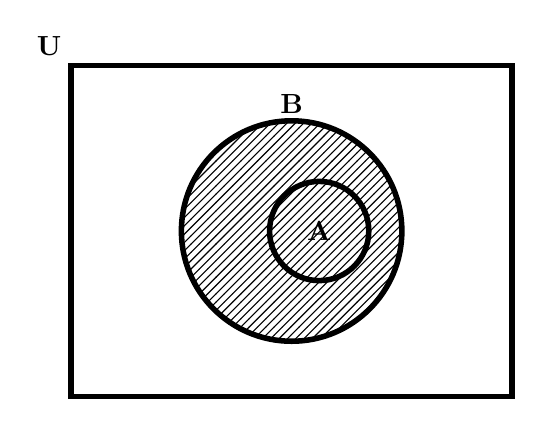
\begin{tikzpicture}[scale=0.7]
    \draw[line width=2pt] (0,0) rectangle (8,6);
    \draw[line width=2pt] (4,3) circle(2);      % B
    \draw[line width=2pt] (4.5,3) circle(0.9);  % A dentro de B
    \begin{scope}
    \clip (4,3) circle(2);
    \fill[pattern=north east lines] (0,0) rectangle (8,6);
    \end{scope}

    \node at (4.5,3) {$\mathbf{A}$};
    \node at (4,5.3) {$\mathbf{B}$};
    \node at (0,6)[above left] {$\mathbf{U}$};
    \end{tikzpicture}
    \end{center}}
    \column{0.4\textwidth}
    
    \only<3>{\begin{center}
    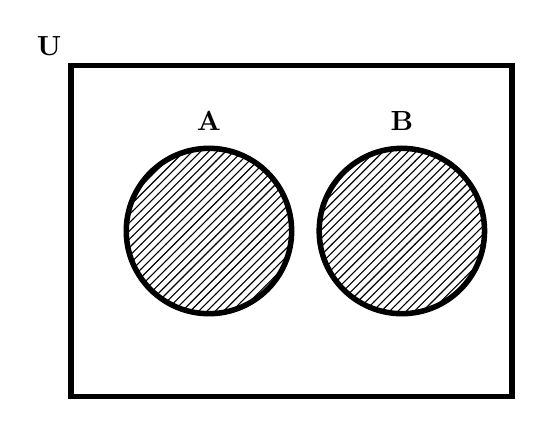
\begin{tikzpicture}[scale=0.7]
    \draw[line width=2pt] (0,0) rectangle (8,6);
    \draw[line width=2pt] (2.5,3) circle(1.5); % A
    \draw[line width=2pt] (6,3) circle(1.5);   % B
    \begin{scope}
    \fill[pattern=north east lines] (2.5,3) circle(1.5);
    \fill[pattern=north east lines] (6,3) circle(1.5);
    \end{scope}
    \node at (2.5,5) {$\mathbf{A}$};    
    \node at (6,5) {$\mathbf{B}$};
    \node at (0,6)[above left] {$\mathbf{U}$};
    \end{tikzpicture}
    \end{center}}
\end{columns}
\end{frame}

\begin{frame}[t]{Ejemplo de unión} 
Considera los siguientes conjuntos
\begin{itemize}
    \item $A=\{2,4,6,8,10\}$ (Pares)
    \item $B=\{1,2,3,4,5\} $ (Números del 1 al 5)
\end{itemize}
Hallar $A\cup B$.
\end{frame}

\begin{frame}[t]{Intercepción} 
\large
\begin{block}{Definión}
\textbf{La intersección} de $A$ y $B$ es el conjunto formado por los elementos comúnes de ambos conjuntos.
$$A\cap B = \{x: x\in A \text{ y } x\in B\}.$$
\end{block}
\only<2->{
\begin{center}
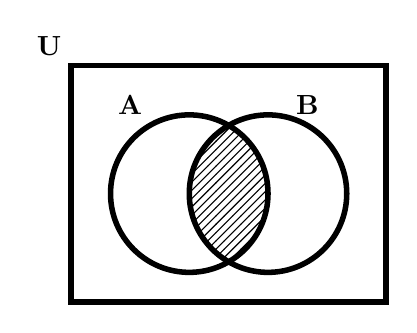
\begin{tikzpicture}[scale= 0.5]

\draw[line width=2pt] (0,0) rectangle (8,6);

\draw[line width=2pt] (3,2.75) circle(2); % A
\draw[line width=2pt] (5,2.75) circle(2); % B

\begin{scope}

\clip (3,2.75) circle(2);
\clip (5,2.75) circle(2);

\fill[pattern=north east lines] (0,0) rectangle (8,6);

\end{scope}

\node at (1.5,5) {$\mathbf{A}$};
\node at (6,5) {$\mathbf{B}$};
\node at (0,6)[above left] {$\mathbf{U}$};

\end{tikzpicture}
\end{center}}
\end{frame}

\begin{frame}{Otros casos de intersección}
\begin{columns}[onlytextwidth]
    \column{0.5\textwidth}
\only<2->{\begin{center}
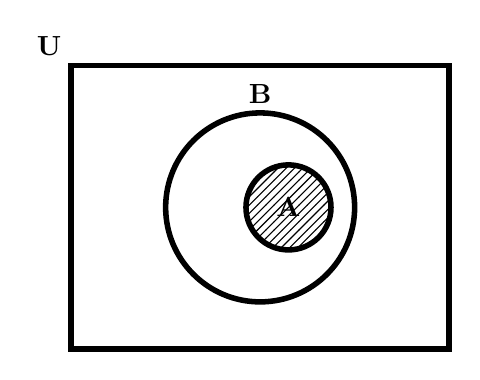
\begin{tikzpicture}[scale= 0.6]

\draw[line width=2pt] (0,0) rectangle (8,6);

\draw[line width=2pt] (4,3) circle(2);      % B
\draw[line width=2pt] (4.6,3) circle(0.9);  % A dentro de B

\begin{scope}

\clip (4.6,3) circle(0.9);
\fill[pattern=north east lines] (0,0) rectangle (8,6);

\end{scope}

\node at (4.6,3) {$\mathbf{A}$};
\node at (4,5.4) {$\mathbf{B}$};
\node at (0,6)[above left] {$\mathbf{U}$};

\end{tikzpicture}
\end{center}}
    \column{0.5\textwidth}
    
    \only<3->{\begin{block}{Definición}
        Cuando $ A$ y $ B$ no tienen elementos en común, se les llama \textbf{disjuntos} y en este caso $A\cap B =\varnothing$.
    \end{block}}
    
\end{columns}
    
\end{frame}


\begin{frame}[t]{Ejemplo de intercepción} 
\large
Considera los siguientes conjuntos
\begin{itemize}
    \item $A=\{2,4,6,8,10\}$ (Pares)
    \item $B=\{1,2,3,4,5\} $ (Números del 1 al 5)
\end{itemize}
Hallar $A\cap B.$
\end{frame}

\begin{frame}[t]{Diferencia}
\large
\begin{block}{Definión}
\textbf{La diferencia} de $A$ y $B$ es el conjunto formado por los elementos de $A$ que no están en $B$.
$$A-B = \{x: x\in A \text{ y } x\notin B\}.$$
\end{block}
\only<2->{
\begin{center}

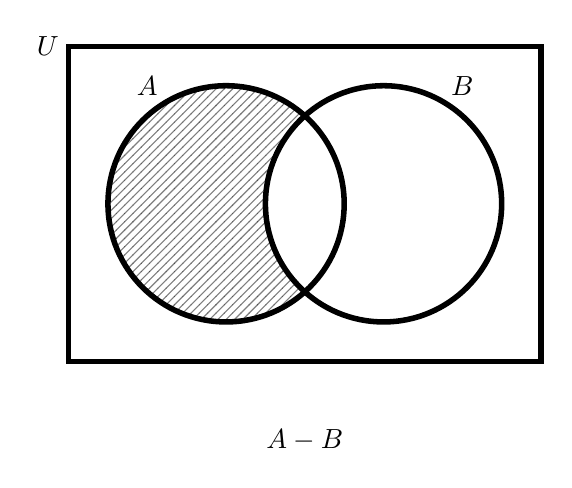
\begin{tikzpicture}[scale=1]

% Rectángulo del conjunto universal
\draw[line width=2pt] (1,0) rectangle (7,4);

% Región A - B
\begin{scope}
\clip (3,2) circle (1.5);          % limitar a A
\fill[pattern=north east lines, opacity=0.5] (3,2) circle (1.5);
\end{scope}

\begin{scope}
\clip (5,2) circle (1.5);          % eliminar la intersección
\fill[white, ] (3,2) circle (1.5);
\end{scope}

% Bordes de los conjuntos
\draw[line width=2pt] (3,2) circle (1.5);
\draw[line width=2pt] (5,2) circle (1.5);

% Etiquetas
\node at (1,4)[left] {$U$};
\node at (2,3.5) {$A$};
\node at (6,3.5) {$B$};

% Texto inferior
\node at (4,-1) {$A - B$};

\end{tikzpicture}

\end{center}}

\end{frame}
\begin{frame}[t]{La diferencia no es conmutativa}
    \begin{alertblock}{Observación}
    No son iguales $A-B$ y $B-A$.
\end{alertblock}

\only<2>{\begin{columns}[onlytextwidth]
\column{0.5\textwidth}
\begin{center}

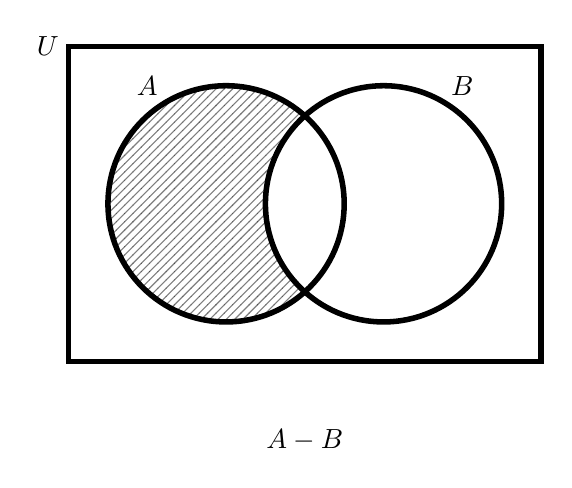
\begin{tikzpicture}[scale=1]

% Rectángulo del conjunto universal
\draw[line width=2pt] (1,0) rectangle (7,4);

% Región A - B
\begin{scope}
\clip (3,2) circle (1.5);          % limitar a A
\fill[pattern=north east lines, opacity=0.5] (3,2) circle (1.5);
\end{scope}

\begin{scope}
\clip (5,2) circle (1.5);          % eliminar la intersección
\fill[white] (3,2) circle (1.5);
\end{scope}

% Bordes de los conjuntos
\draw[line width=2pt] (3,2) circle (1.5);
\draw[line width=2pt] (5,2) circle (1.5);

% Etiquetas
\node at (1,4)[left] {$U$};
\node at (2,3.5) {$A$};
\node at (6,3.5) {$B$};

% Texto inferior
\node at (4,-1) {$A - B$};

\end{tikzpicture}

\end{center}

\column{0.5\textwidth}
   \begin{center}

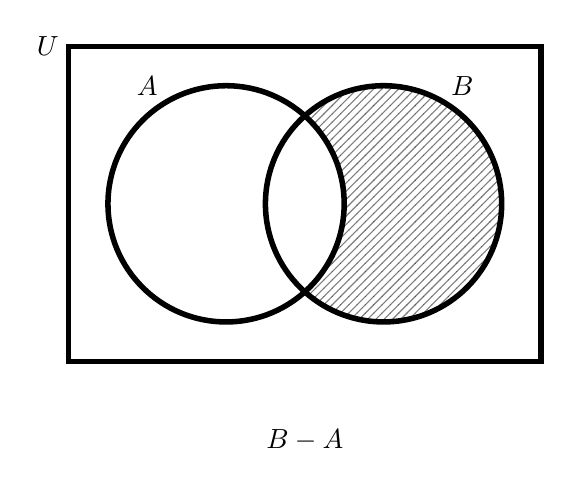
\begin{tikzpicture}[scale=1]

% Rectángulo del conjunto universal
\draw[line width=2pt] (1,0) rectangle (7,4);

% Región B - A
\begin{scope}
\clip (5,2) circle (1.5);      % limitar a B
\fill[pattern=north east lines, opacity=0.5] (5,2) circle (1.5);
\end{scope}

\begin{scope}
\clip (3,2) circle (1.5);      % eliminar intersección con A
\fill[white] (5,2) circle (1.5);
\end{scope}

% Bordes de los conjuntos
\draw[line width=2pt] (3,2) circle (1.5);
\draw[line width=2pt] (5,2) circle (1.5);

% Etiquetas
\node at (1,4)[left] {$U$};
\node at (2,3.5) {$A$};
\node at (6,3.5) {$B$};

% Texto inferior
\node at (4,-1) {$B - A$};

\end{tikzpicture}

\end{center}
\end{columns}}

\end{frame}

\begin{frame}{Otros casos de diferencia}
    \begin{columns}[onlytextwidth]
        \column{0.5\textwidth}
        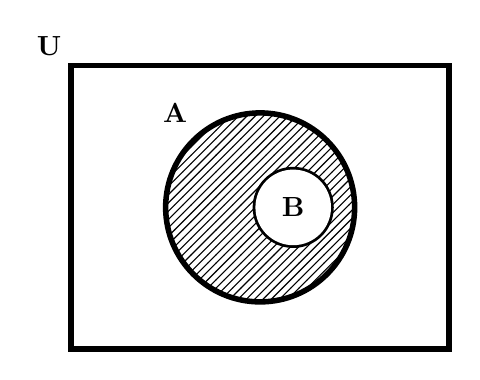
\begin{tikzpicture}[scale=0.6]

\draw[line width=2pt] (0,0) rectangle (8,6);

\draw[line width=2pt] (4,3) circle(2);      % Conjunto A
\draw[line width=2pt] (4.7,3) circle(0.8);  % Conjunto B dentro de A

\begin{scope}

\clip (4,3) circle(2); % recorte en A
\fill[pattern=north east lines] (0,0) rectangle (8,6);

\fill[white] (4.7,3) circle(0.8); % quitar B

\end{scope}

\node at (2.2,5) {$\mathbf{A}$};
\node at (4.7,3) {$\mathbf{B}$};
\node at (0,6)[above left] {$\mathbf{U}$};

\end{tikzpicture}
        \column{0.5\textwidth}
        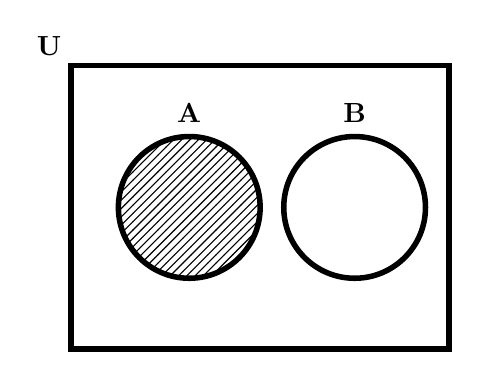
\begin{tikzpicture}[scale=0.6]

\draw[line width=2pt] (0,0) rectangle (8,6);

\draw[line width=2pt] (2.5,3) circle(1.5);  % A
\draw[line width=2pt] (6,3) circle(1.5);    % B (separado)

\begin{scope}

\clip (2.5,3) circle(1.5);
\fill[pattern=north east lines] (0,0) rectangle (8,6);

\end{scope}

\node at (2.5,5) {$\mathbf{A}$};
\node at (6,5) {$\mathbf{B}$};
\node at (0,6)[above left] {$\mathbf{U}$};

\end{tikzpicture}
    \end{columns}
\end{frame}

\begin{frame}[t]{Ejemplo diferencia}
    Considera los siguientes conjuntos
\begin{itemize}
    \item $A=\{2,4,6,8,10\}$ (Pares)
    \item $B=\{1,2,3,4,5\} $ (Números del 1 al 5)
\end{itemize}
Hallar $A-B$ y $B-A$.
\end{frame}




\begin{frame}[t]{Complemento} 
\begin{block}{Definión}
Dado un conjuntos $A$ \textbf{el complemento} de $A$ denotada por $A^c$ es el conjunto $U-A$. Es decir, todos los elementos que no pertencen a $A$.
$$A^c = \{x: x\notin A\}.$$
    
\end{block}
\only<2>{
\begin{center}
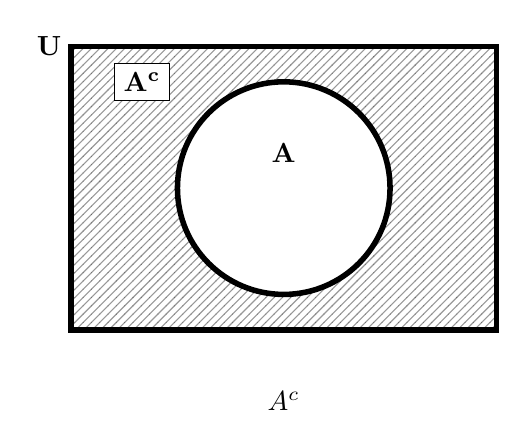
\begin{tikzpicture}[scale=0.9]

% Rectángulo del conjunto universal
\draw[line width=2pt] (1,0) rectangle (7,4);

% Región A^c
\fill[pattern=north east lines, opacity=0.4, even odd rule]
(1,0) rectangle (7,4)
(4,2) circle (1.5);

% Bordes de los conjuntos
\draw[line width=2pt] (4,2) circle (1.5);

% Etiquetas
\node at (1,4)[left] {$\mathbf{U}$};
\node at (4,2.5) {$\mathbf{A}$};
\node at (2,3.5)[draw, rectangle, fill=white] {$\mathbf{A^c}$};

% Texto inferior
\node at (4,-1) {$A^{c}$};

\end{tikzpicture}

\end{center}}
\end{frame}

\begin{frame}[t]{Ejemplo de complemento} 
\Large
Considera los siguientes conjuntos
\begin{itemize}
    \item $U=\{1,2,3,4,5,6,7,8,9,10\}$
    \item $A=\{2,4,6,8,10\}$ (Pares)
    \item $B=\{1,2,3,4,5\} $ (Números del 1 al 5)
\end{itemize}
Hallar $A^c$ y $B^c$.
\end{frame}

\begin{frame}[t]{Para pensar}
\large
Sea $A$ un conjunto cualquiera y $U$ el conjunto universo. ¿Cuál es el resultado de las siguientes operaciones?

\begin{columns}[onlytextwidth]
\column{0.5\textwidth}
\begin{enumerate}
    \item $A\cup A =$
    \item $A\cap A =$
    \item $A\cup A^c =$
    \item $A\cap A^c =$
    \item $ A\cap U = $
    \item $A \cup U =$
    \item $(A^c)^c =$
\end{enumerate}

\column{0.5\textwidth}
   \begin{enumerate}
    \item $A\cup \varnothing =$
    \item $A\cap \varnothing = $
    \item $\varnothing^c =$
    \item $U^c =$
    \item $ \varnothing\cap U^c =$
    \item $\varnothing\cup U =$
\end{enumerate} 
\end{columns}
\end{frame}

\begin{frame}[t]{Diferencia Simétrica}
\begin{block}{Definición}
    La diferencia simétrica entre dos conjuntos \textbf{A} y \textbf{B} es el conjunto de elementos que pertenecen a uno de los dos conjuntos, pero no a ambos al mismo tiempo. Es decir, son los elementos que están solo en \textbf{A }o solo en \textbf{B}.
    $$A\Delta B = (A-B)\cup (B-A)$$
    \end{block}
    \begin{center}
        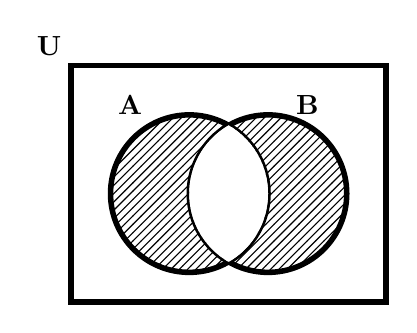
\begin{tikzpicture}[scale=0.5]

\draw[line width=2pt] (0,0) rectangle (8,6);

\draw[line width=2pt] (3,2.75) circle(2); % A
\draw[line width=2pt] (5,2.75) circle(2); % B

% Parte A-B
\begin{scope}
\clip (3,2.75) circle(2);
\fill[pattern=north east lines] (0,0) rectangle (8,6);
\fill[white] (5,2.75) circle(2);
\end{scope}

% Parte B-A
\begin{scope}
\clip (5,2.75) circle(2);
\fill[pattern=north east lines] (0,0) rectangle (8,6);
\fill[white] (3,2.75) circle(2);
\end{scope}

\node at (1.5,5) {$\mathbf{A}$};
\node at (6,5) {$\mathbf{B}$};
\node at (0,6)[above left] {$\mathbf{U}$};

\end{tikzpicture}
    \end{center}
\end{frame}


\begin{frame}[t]{Ejemplo}
\small

En una preparatoria, se han formado dos clubes de alto rendimiento. Debido a la intensidad de las actividades, la dirección ha prohibido por reglamento que un alumno pertenezca a ambos clubes al mismo tiempo para evitar el agotamiento académico.

\begin{center}
    \textbf{Club de Robótica ($A$):} $\{ \text{Ana, Beto, Carla, Diego, Elena} \}$ \\
    \textbf{Club de Debate ($B$):} $\{ \text{Carla, Diego, Fabián, Gloria, Hugo} \}$
\end{center}

\textbf{El Problema:} \\
La dirección necesita identificar quiénes son los alumnos que están en una \textbf{situación legal} (aquellos que cumplen la norma de estar en un solo club) para entregarles su credencial. Aquellos que se encuentren en ambos clubes serán citados a coordinación.
\begin{enumerate}[A)]
    \item Identifica el conjunto de la intersección ($A \cap B$). ¿Qué representan estos alumnos en el contexto del problema?
    \item Calcula la \textbf{Diferencia Simétrica} ($A \Delta B$). Escribe la lista de nombres de los alumnos que recibirán su credencial.
    \item Utilizando un Diagrama de Venn, sombrea la región que representa a los alumnos con situación legal.
    
\end{enumerate}

\end{frame}


\begin{frame}{Cardinalidad de un Conjunto}
\begin{block}{Definición}
    La cardinalidad de un conjunto es el número de elementos que tiene el conjunto. Notación $\#(A)$.
\end{block}

\begin{columns}[onlytextwidth]
    \column{0.5\textwidth}
\only<2->{ \textbf{Ejemplo 1:}
$A=\{2,4,6,8\}$
\only<3->{
\centering{
$\Rightarrow
\#(A)=4
$}
}}


\only<4->{
\textbf{Ejemplo 2:}
$ B=\{a,e,i,o,u\}$
\only<5->{
\centering{$\Rightarrow\#(B)=5$}
}}


\column{0.5\textwidth}

\only<6->{
    \textbf{Ejemplo 3:}
    $C=\{1,3,3,5,5,7\}$}
    \only<7->{
    \centering{$\Rightarrow\#(C)=4$}}

    \only<8->{\textbf{Ejemplo 4:}
$ A\cup C =\{1, 2, 3, 4, 5, 6, 7, 8\}$}
\only<9->{
\centering{$
\Rightarrow\#(A\cup C)= 8.
$}}
\end{columns}

\end{frame}

\begin{frame}{Cardinal de la Unión}
\begin{block}{Propiedad}
    $$\#(A\cup B) = \#(A)+\#(B)-\#(A\cap B)$$
\end{block}

\end{frame}


\begin{frame}{Conjunto Potencia}
\only<2->{
\begin{block}{Definición}
    El conjunto potencia es el conjunto que tiene por elementos a todos los subconjuntos de un conjunto. Es decir, el conjunto potencia $\mathbf{P}(\mathbf{A})$ es el conjunto formado por todos los subconjuntos de $\mathbf{A}$.
    \only<3->{$$\mathbf{P(A)}=\{B: B\subset A\}$$}
\end{block}
}

\only<3->{\begin{alertblock}{Importante}
\begin{enumerate}
\item<4-> Los elementos de $\mathbf{P}(A)$ son conjuntos.
\item<5-> $\varnothing \subset A$
    \item<6-> $A\subset A$
    \item<7-> $ \mathbf{\therefore}\quad   \varnothing , A \in \mathbf{P}(A)$ \pause{$\quad\Rightarrow P(A)\neq \varnothing.$}
\end{enumerate}
\end{alertblock}}
\end{frame}

\begin{frame}{Ejemplo}
   \only<1->{\textbf{Ejemplo:} Sea $A=\{1,2\}$.}

\only<2->{Los subconjuntos de $A$ son:

$$
\varnothing,\{1\},\{2\},\{1,2\}.
$$}
\only<3->{
El \textbf{conjunto potencia} de $A$ es de $A$.

$$
\mathbf{P}(A)=\{\varnothing,\{1\},\{2\},\{1,2\}\}.
$$} 
\end{frame}

\begin{frame}{Cardinal del Conjunto Potencia}
\pause{
\begin{block}{Propiedad}
$$\#\mathbf{P}(A) = 2^{\#A}.$$
\end{block}}
\pause{
Ejemplo: Sea $A=\{1,2\}$.}

\pause{
$$\mathbf{P}(A)=\{\varnothing,\{1\},\{2\},\{1,2\}\}.$$}
\pause{
$$\Rightarrow \#\mathbf{P}(A) = 2^2=4.$$}
\end{frame}

\begin{frame}{Producto Cartesiano}
\pause{
\begin{block}{Definición}  
Dados dos conjuntos $A$ y $B$, se define el producto cartesiano como el conjunto de todos los pares ordenados $(a, b)$ con $a \in A$ y $b \in B$:

\[
A \times B = \{(a, b) \mid a \in A, \; b \in B\}.
\]  
\end{block}}

\pause{
\begin{alertblock}{Observaciones:}
    \begin{enumerate}[<+->]
    \item Dos pares ordenados $(a, b)$ y $(c, d)$ son iguales si y solo si $a = c$ y $b = d$.
    \item El par ordenado $(a, b)$ es distinto de $(b, a)$, salvo que $a = b$.
    \item Es posible que ambos elementos coincidan, por ejemplo $(a, a)$.
\end{enumerate}
\end{alertblock}}

\end{frame}

\begin{frame}{Ejemplo}
\begin{itemize}
\item Ejemplo 1. Sea $A = \{1, 2\}$ y $B = \{3, 4, 5\}$.\pause{
\[\Rightarrow
A \times B = \{(1, 3), (1, 4), (1, 5), (2, 3), (2, 4), (2, 5)\}.
\]}
\end{itemize}
\end{frame}

\section{Interpretación de Zonas de Conjuntos}

\begin{frame}{Interpretación de Zonas de Conjuntos}
	\only<1->{
	\begin{columns}[onlytextwidth]
		\column{0.5\textwidth}
			\begin{center}
				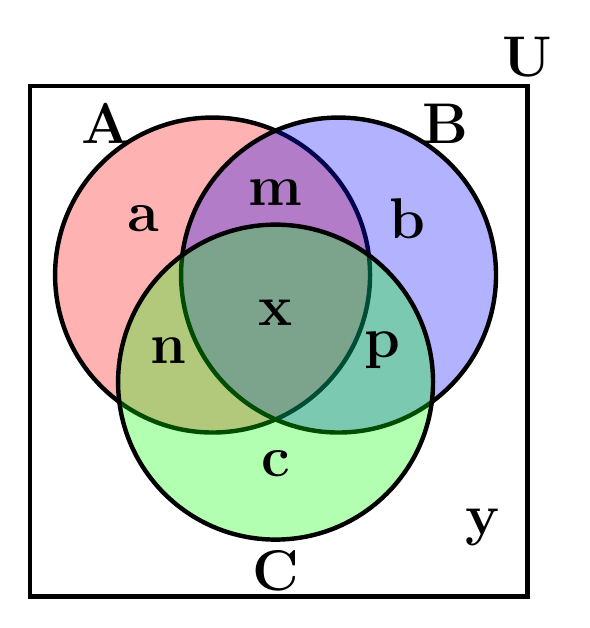
\begin{tikzpicture}[scale=0.8]
					
					% 1. Definición del Conjunto Universal (U)
					\draw[ultra thick] (-3.9,-4.4) rectangle (4,3.7);
					\node at (4, 3.7)[above] {\textbf{\huge U}};\pause
					
					% 2. Estilo de los círculos
					\tikzset{set/.style={draw, circle, minimum size=4cm, ultra thick, fill opacity=0.3}}
					
					% 3. Posicionamiento de los círculos (Conjuntos A, B y C)
					\node[set, fill=red] (A) at (-1, 0.7) {};
					\node at (-2.7, 3.1) {\textbf{\huge A}};\pause
					\node[set, fill=blue] (B) at (1, 0.7) {};
					\node at (2.7, 3.1) {\textbf{\huge B}};\pause
					\node[set, fill= green] (C) at (0, -1) {};
					\node at (0, -4) {\textbf{\huge C}};
					
					\pause
					% 5. Etiquetas de las regiones (Elementos/Variables)
					% Regiones individuales
					\node at (-2.1, 1.6) {\huge $\mathbf{a}$};
					\node at (2.1, 1.6)  {\huge $\mathbf{b}$};
					\node at (0, -2.3)   {\huge $\mathbf{c}$};
					
					% Intersecciones de dos conjuntos
					\node at (0, 2.0)    {\huge $\mathbf{m}$};
					\node at (-1.7, -0.5) {\huge $\mathbf{n}$};
					\node at (1.7, -0.5)  {\huge $\mathbf{p}$};
					
					% Intersección de los tres conjuntos
					\node at (0, 0.1)    {\huge $\mathbf{x}$};
					
					% Elemento fuera de los conjuntos (en el Universal)
					\node at (3.3, -3.3) {\huge $\mathbf{y}$};
					
				\end{tikzpicture}
			\end{center}
		\column{0.5\textwidth}}
		\only<5->{
		\pause
		\begin{block}{\textbf{\underline{Interpretación:}}}
		\pause
			\begin{enumerate}
			\item $\mathbf{A:\pause a+m+n+x}$
			\item \textbf{Solo} $\mathbf{A: \pause a}$
			\item $\mathbf{A}$ y $\mathbf{B: \pause  m+x}$
			\item \textbf{Solo} $\mathbf{A}$ y $\mathbf{B: \pause m}$
			\item $\mathbf{A \text{ o } B: \pause a+m+b+n+x+p}$
			\item \textbf{Solo} $\mathbf{A \text{ o } B} :\, \pause \mathbf{a+m+b}$
			\item \textbf{Solamente Uno} :\,\,\pause  $\mathbf{a+b+c}$
			\item \textbf{Solo Dos} : \pause$\mathbf{m+n+p}$
			\item \textbf{Ninguno} :\, \pause $\mathbf{y}$ 
		\end{enumerate}	
		\end{block}
		}
	\end{columns}
		\end{frame}





\end{document}
